\documentclass{beamer}
\usepackage{mathtools}
\usepackage{listings}
\usepackage{graphicx}
\usetheme{metropolis}
%\usetheme[secheader]{Boadilla} %Antibes,CambridgeUS
%\usecolortheme{spruce} 
% color : MIT red: beaver
%         Michigan green : spruce
%         black and white: dove , more shadow: seagull
\usefonttheme[]{structurebold}

\title{Variable Selection For Discrete Competing Risks Models}
\date{\today}
\author{Jingwei Zhang, Lupengkong, 
    Chunlong Luo,
    Quanfeng Yang,
    Yiqing Lu
    \\
    {\ttfamily skykiny@outlook.com}
}
%\institute{Centre for Modern Beamer Themes}

\begin{document}
    \maketitle
    
    %\begin{frame}{Content}{}
    %    \tableofcontents
    %\end{frame}
    
    \section{Statistical Model}
    \subsection{The Discrete Competing Risk Model}
    \begin{frame}{The Discrete Competing Risk Model}%{sub section}
        \begin{itemize}
            \item Consider an example involving multiple causes of failure.
            \item For a patient who took surgery, we want to study the occurrence of different types of events, such as disease recurrence and death.
            \item This patient is followed up for several times. In every follow-up, we care about whether these event happens or not.
            \begin{itemize}
                \item If {\bf one} of these events happens, the follow up will {\bf stop}.
                \item If {\bf none} of these event happens(usually we call this situation {\bf survival}), we {\bf continue} to monitor this patient.
                \item After several times of follow up, the monitor will stop(we call it {\bf censoring}).
            \end{itemize}
        \end{itemize}
    \end{frame}
    
    \begin{frame}{Purpose of the Model}
        This model can be used to:
        \begin{itemize}
            \item study the relationship between a vector of covariates $\mathbf{x}$ and the rate of occurrence of specific types of failure.
            \item estimate the risk of one type of failure after removing others. 
        \end{itemize}
    \end{frame}
    
    \begin{frame}{Example of State Transition}
        \begin{itemize}
            \item $T \in \{1,\dots,k\}$ indicates the {\bf first time} of happening of event, $C$ indicates the time of censoring.
            \item $Y_t$ indicates the status of the object on time $t$. $R_1,\dots,R_m$ indicates $m$ events and $S$ indicates survival.
        \end{itemize}
        
        \begin{figure}
            \centering
            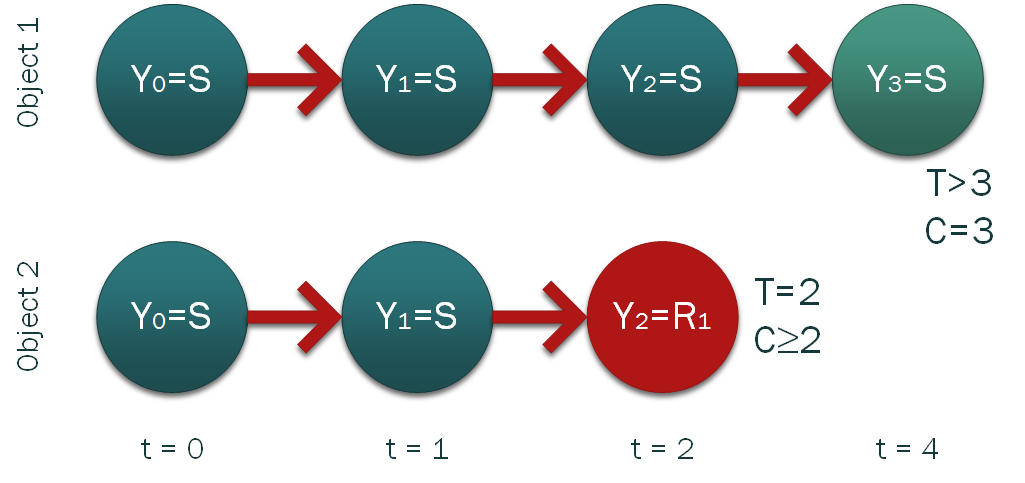
\includegraphics[width=\linewidth]{./two_patient.png}
            %\caption{Figure for $10^4$}
        \end{figure}
    \end{frame}
    
    \begin{frame}{Graph of State Transition}
        \begin{itemize}
            \item $\lambda_r(t|\mathbf{x})$ represents the transitional probability from state $S$ to state $R_r$. $r=0$ represents no event happens.
            \item  We call $\lambda_r(t|\mathbf{x})$ cause-specific discrete hazard function.
            \item Both $\mathbf{x}$ and $t$ affects probability of transition.
        \end{itemize}
        \begin{figure}
            \centering
            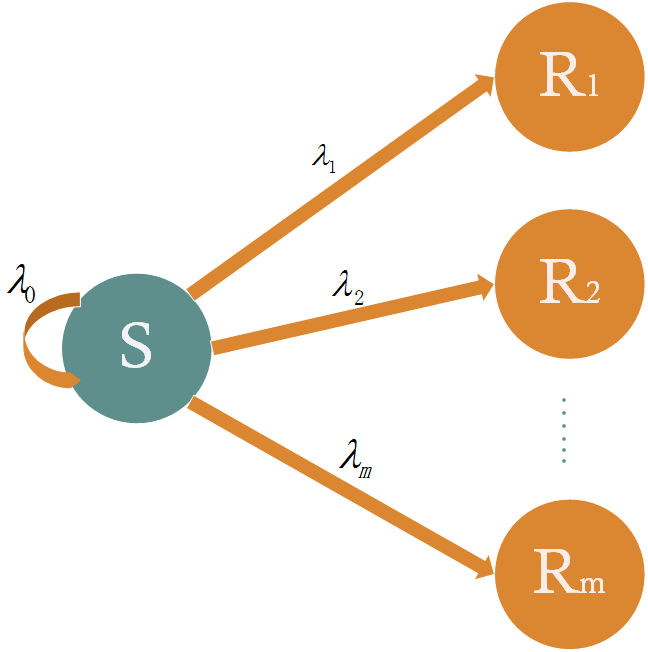
\includegraphics[scale=0.3]{./transition.png}
            %\caption{Figure for $10^4$}
        \end{figure}
    \end{frame}
    
    \begin{frame}{Hazard Functions}
        The {\bf cause-specific hazard function}:
        \begin{align*}
        \lambda_r(t|\mathbf{x}) &= P(Y_t = R_r | Y_{t-1} = S, \mathbf{x}) \\
        &= P(T = t, R = r | T \geq t, \mathbf{x})
        \end{align*}
        Summing up for all events, we get {\bf hazard function}:
        \begin{equation*}
        \lambda(t|\mathbf{x}) = \sum_{r = 1}^{m} \lambda_r(t|\mathbf{x}) = P(T = t | T \geq t, \mathbf{x})
        \end{equation*}
        For survival, we have:
        \begin{align*}
        \lambda_0(t|\mathbf{x}) 
        = 1 - \lambda(t|\mathbf{x}) 
        = 1- \sum_{r = 1}^{m} \lambda_r(t|\mathbf{x})
        \end{align*}
    \end{frame}
    
    \begin{frame}{Unconditional Probability}
        The {\bf survival function}, which indicates the unconditional probability of no event happening:
        \begin{align*}
        S(t|\mathbf{x}) = P(T > t | \mathbf{x}) = \prod_{j = 1}^{t} (1-\lambda(j|\mathbf{x}))
        \end{align*}
        The unconditional probability of one event happening on time $t$:
        \begin{align*}
            P(T= t|\mathbf{x}) &= \lambda(t|\mathbf{x}) \prod_{j = 1}^{t-1} (1-\lambda(j|\mathbf{x})) \\
            &= \lambda(t|\mathbf{x}) S(t-1|\mathbf{x})
        \end{align*}
    \end{frame}
    
    \begin{frame}{The Multinomial Logit Model}
        To model the influence of $\mathbf{x}$ on transitional probability $\lambda_r$, multinomial logit model is used:
        \begin{align*}
        \lambda_r(t|\mathbf{x}) = \frac{ \exp{ (\beta_{0tr}+\mathbf{x}^\mathsf{T} \mathbf{\gamma_r} ) } }{ 1+ \sum_{s=1}^{m} \exp{ (\beta_{0ts}+\mathbf{x}^\mathsf{T} \mathbf{\gamma_s}) }  }
        \end{align*}
        where $t = 1,\dots, q$, and $r = 1,\dots, m$.
        \begin{itemize}
            \item $\beta_{01r}, \dots, \beta_{0qr}$ determine the
            cause-specific baseline hazard functions.
            \item $\mathbf{\gamma_r}$ contains the cause-specific effects of covariates.
        \end{itemize}
        For survival, we have:
        \begin{align*}
        \lambda_0(t|\mathbf{x})= 1 - \sum_{r=1}^{m} \lambda_r(t|\mathbf{x}) = \frac{ 1 }{ 1+ \sum_{s=1}^{m} \exp{ (\beta_{0ts}+\mathbf{x}^\mathsf{T} \mathbf{\gamma_s}) }  }
        \end{align*}
        
    \end{frame}
    
    \subsection{Estimation}
    \begin{frame}{Original Data}
        Data is given by $(t_i,r_i,\delta_i, \mathbf{x}_i)$, $i = 1,\dots,n$
        \begin{itemize}
            \item $t_i = min(Ti,Ci)$ is the observed discrete time, which is the minimum of survival time $T_i$ and censoring time $C_i$.
            \item We always assume {\bf random censoring}, that is, $T_i$ and $C_i$ are assumed to be independent
            \item $r_i \in \{1,\dots,m\}$ indicates the type of the terminating event
            \item $\mathbf{x}_i$ is the covariate vector
            \item $\delta_i$ denotes the censoring indicator with
            \begin{align*}
            \delta_i = \begin{cases}
            1, &\quad \text{if event occured on time }t_i \\
            0, &\quad \text{if it censores on time }t_i
            \end{cases}
            \end{align*}
        \end{itemize}
    \end{frame}
    
    \begin{frame}{Liklihood Function}
        The likelihood contribution of the $i$-th observation is given by($\mathbf{x}$ is is omitted):
        \begin{align*}
        L_i = P(T_i = t_i,R_i = r_i)^{\delta_i}P(T_i > t_i)^{1-\delta_i} P(C_i \geq t_i)^{\delta_i} P(C_i = t_i)^{1-\delta_i}
        \end{align*}
        
        Under the assumption that censoring does not depend on the parameters that determine the survival time ({\bf non-informative censoring}), $L_i$ can be reduced to
        \begin{align*}
        L_i 
        &= P(T_i = t_i,R_i = r_i|\mathbf{x})^{\delta_i}P(T_i > t_i|\mathbf{x})^{1-\delta_i}  \\
        &=\lambda_{r_i}(t_i|\mathbf{x}_i)^{\delta_i}
        (1-\lambda(t_i|\mathbf{x}_i))^{1-\delta_i}
        \prod_{t=1}^{t_i-1}(1-\lambda(t|\mathbf{x}_i)) \label{log liklihood using delta}
        \end{align*}
    \end{frame}
    
    \begin{frame}{Response Vector}
         For an alternative form of the likelihood, indicators for the transition to the
         next period are defined by
         \begin{align}
         y_{itr} = \begin{cases}
         1, &\quad \text{if event of type }r\text{ occured on time }t \\
         0, &\quad \text{if event of type }r\text{ did not occure on time }t
         \end{cases}
         \end{align}
         and
         \begin{align}
         y_{it0} = \begin{cases}
         1, &\quad \text{if no events occured on time }t \text{ (survive)} \\
         0, &\quad \text{if one of the } m\text{ events occures on time }t
         \end{cases}
         \end{align}
         where $i \in R_t$ and $r=1,\dots,m$. These indicator variables are gathered in the vector $\mathbf{y}_{it}^\mathsf{T}  = (y_{it0},y_{it1},...,y_{itm})$ denoting the response vector of object $i$, $i = 1,\dots,n$, $t = 1,\dots,t_i$.
    \end{frame}
    
     \begin{frame}{Response Vector - Example}
         \begin{align*}
         \mathbf{y}_{it} = \begin{bmatrix}
         1 \\ 0 \\ \vdots \\ 0
         \end{bmatrix}
         \end{align*}
         where $y_{it0} = 1$ while others are $0$. This vector indicates that on time $t$, the object $i$ survives.
         \begin{align*}
         \mathbf{y}_{it} = \begin{bmatrix}
         0 \\ \vdots\\1\\ \vdots \\ 0
         \end{bmatrix}
         \end{align*}
         where $y_{itj} = 1$ while others are $0$. This vector indicates thar on time $t$, event $j$ happens.
     \end{frame}
     
     \begin{frame}{Rewrite the Liklihood Function}
         Using response vector, the likelihood function $Li$ can be rewritten as:
         \begin{align*}
         L_i = \prod_{t = 1}^{t_i}  (\prod_{r = 0}^{m} \lambda_{r}(t_i|\mathbf{x}_i)^{y_{itr}}) 
         \end{align*}
         This is actually a multinomially distribution with $\mathbf{y}_{it}^\mathsf{T}  = (y_{it0},y_{it1},...,y_{itm}) \sim \mathcal{M}(1, ( \lambda_0(t|\mathbf{x}),\lambda_1(t|\mathbf{x}),\dots,\lambda_m(t|\mathbf{x}) ) )$
     \end{frame}
    
     \begin{frame}{Log Liklihood Function}
         The total log-liklihood is given by
         \begin{align*}
         l = \sum_{i=1}^{n} \sum_{t = 1}^{t_i} \sum_{r=0}^{m}
         y_{itr} \log\lambda_r(t|\mathbf{x})
         \end{align*}
         where $\lambda_r(t|\mathbf{x})$ is given by multinomial logit model:
         \begin{align*}
         \lambda_r(t|\mathbf{x}) = \frac{ \exp{ ( \eta_{itr} ) } }{ 1+ \sum_{s=1}^{m} \exp{ (\eta_{its}) }  }
         \end{align*}
         where $\eta_{itr} = \beta_{0tr}+\mathbf{x}^\mathsf{T} \mathbf{\gamma_r}$.\\
         This ML estimates can be easily computed by using statistical software for multinomial regression models.
     \end{frame}
\end{document}


